\documentclass{beamer}

\usepackage [french] {babel}
\usepackage [T1] {fontenc}
\usepackage [utf8] {inputenc}
\usepackage{booktabs}
\usepackage{graphicx}
\usepackage{xcolor}
\usepackage{colortbl}

\graphicspath{{./Images/}}

\title{TIPE}
\author{Maxence}
\date{\today}

\begin{document}

\frame{\titlepage}

\section[Outline]{}
\frame{\tableofcontents}

\section{Introduction}
\subsection{Overview of un neurone\footnote{a neuron in english}.}
\frame{
\begin{figure}[htbp]
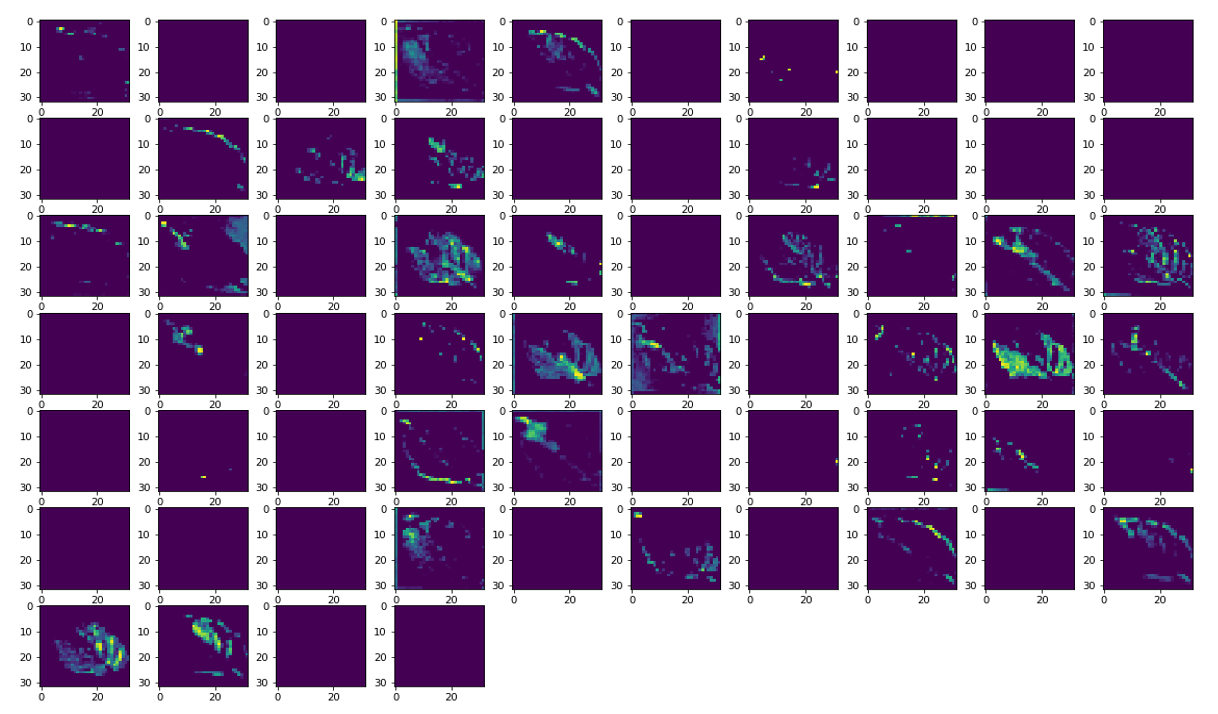
\includegraphics[scale=0.5]{image_base}
\caption{This is a caption}
\end{figure}
}

\begin{frame}
% Table generated by Excel2LaTeX from sheet 'Base'
\begin{table}[htbp]
  \centering
  \caption{Add caption}
  \resizebox*{3cm}{!}{
    \begin{tabular}{|rrr|}
    \toprule
    \rowcolor[rgb]{ .439,  .678,  .278} \multicolumn{1}{|l}{\textcolor[rgb]{ 1,  1,  1}{\textbf{Colonne1}}} & \multicolumn{1}{l}{\textcolor[rgb]{ 1,  1,  1}{\textbf{Train Accuracy}}} & \multicolumn{1}{l|}{\textcolor[rgb]{ 1,  1,  1}{\textbf{Validation Accuracy}}} \\
    \midrule
    \rowcolor[rgb]{ .886,  .937,  .855} 0     & 0,572103441 & 0,78022778 \\
    \midrule
    1     & 0,8095209 & 0,852192879 \\
    \midrule
    \rowcolor[rgb]{ .886,  .937,  .855} 2     & 0,876869977 & 0,862127483 \\
    \midrule
    3     & 0,924414039 & 0,868912041 \\
    \midrule
    \rowcolor[rgb]{ .886,  .937,  .855} 4     & 0,952516496 & 0,895081162 \\
    \midrule
    5     & 0,966204345 & 0,892415822 \\
    \midrule
    \rowcolor[rgb]{ .886,  .937,  .855} 6     & 0,97092849 & 0,878604293 \\
    \midrule
    7     & 0,974259555 & 0,899442673 \\
    \midrule
    \rowcolor[rgb]{ .886,  .937,  .855} 8     & 0,976863921 & 0,891688883 \\
    \midrule
    9     & 0,987160087 & 0,877392769 \\
    \midrule
    \rowcolor[rgb]{ .886,  .937,  .855} 10    & 0,984313488 & 0,882965863 \\
    \midrule
    11    & 0,982981026 & 0,898715794 \\
    \midrule
    \rowcolor[rgb]{ .886,  .937,  .855} 12    & 0,986796677 & 0,865277469 \\
    \midrule
    13    & 0,985343099 & 0,894354224 \\
    \midrule
    \rowcolor[rgb]{ .886,  .937,  .855} 14    & 0,991399646 & 0,865762055 \\
    \midrule
    15    & 0,980073869 & 0,889508128 \\
    \midrule
    \rowcolor[rgb]{ .886,  .937,  .855} 16    & 0,993277192 & 0,881754279 \\
    \midrule
    17    & 0,991036296 & \cellcolor[rgb]{ 1,  .922,  .612}\textcolor[rgb]{ .612,  .341,  0}{0,900896549} \\
    \midrule
    \rowcolor[rgb]{ .886,  .937,  .855} 18    & 0,989461601 & 0,881269693 \\
    \midrule
    19    & 0,994851887 & 0,897261918 \\
    \midrule
    \rowcolor[rgb]{ .886,  .937,  .855} 20    & 0,984555721 & 0,868185103 \\
    \midrule
    21    & 0,992610991 & 0,886600435 \\
    \midrule
    \rowcolor[rgb]{ .886,  .937,  .855} 22    & 0,992489874 & 0,878119707 \\
    \midrule
    23    & 0,987947404 & 0,852677464 \\
    \midrule
    \rowcolor[rgb]{ .886,  .937,  .855} 24    & 0,996184349 & 0,884661973 \\
    \midrule
    25    & 0,99091512 & 0,885146618 \\
    \midrule
    \rowcolor[rgb]{ .886,  .937,  .855} 26    & 0,991520822 & 0,845650613 \\
    \midrule
    27    & 0,99091512 & 0,874727428 \\
    \midrule
    \rowcolor[rgb]{ .886,  .937,  .855} 28    & 0,991884172 & 0,858735144 \\
    \midrule
    29    & 0,990430593 & 0,881511986 \\
    \bottomrule
    \end{tabular}
  }
  \label{tab:addlabel}
\end{table}
\end{frame}

\end{document}

